\chapter{Design}
\label{ch:Design}

Ein wichtiger Teil dieser Arbeit ist die Erstellung eines Datensatzes, welcher zur Klassifikation dienen soll.
Mithilfe einer Smartphone-App soll ein Datensatz eines Studienteilnehmers erstellt und exportiert werden. 
Daraufhin liegen die Daten vor und könnnen in einer Verarbeitungspipeline analysiert, bzw. klassifiziert werden.

Die Studie wurde so konzipiert, Atemaussetzer währrend des Schlafens zu klassifizieren. 
Während der Studie wurde jeder Datensatz im Bett des Teilnehmers aufgezeichnet, was das Wohlbefinden verschärken und somit auch die Qualität der Daten erhöhen soll.

%Dadurch, dass bei der Studie neben den eSense Earpods auch ein PSG-System zum Sammeln der Daten benutzt wird, gestaltet sich die Suche nach Probanden als sehr schwer. 
%Das PSG-System sammelt medizinische Daten, welche nicht ohne Antrag bei der Ethikkommission (REC, \textit{resarch ethics committee}) erhoben werden dürfen. 
Im Rahmen dieser Bachelorarbeit wurde ein Datensatz  nach dem \textit{Sample of Convenience} erstellt.

\section{Studienplanung}
Für die Studie wurde eine Teilnehmeranzahl von 10 Personen gewählt, welche die nötige Vielfältigkeit liefern soll.
Des weiteren wurden pro Teilnehmer ein Datensatz an 3 verschiedene Positionen aufgezeichnet, auf dem Bauch, dem Rücken, sowie auf der Seite liegend.

Eine Fragestellung der Studie war, wie ein Atemaussetzer {\glqq simuliert\grqq} werden soll. 
Es wurde entschieden, dass die Studie ein zentrales Schlafapnoe erkennen soll. 
Demzufolge soll der Studienteilnehmer in einer vordefinierten Reihenfolge einen Atemaussetzer {\glqq simulieren\grqq}, indem er die Luft für eine gewisse Zeit anhält.
Um unterschiedliche Längen von Atemaussetzern aufzuzeichnen wurden $10\si{\s}$, $20\si{\s}$ und $30\si{\s}$ gewählt, in denen der Teilnehmer die Luft anhalten soll. 
Nun muss ein geeigneter Ablauf gewählt werden, wodurch sich die Ereignisse nicht überschneiden.
Auf der Suche, wie Lange die Regeneration dauere, nachdem eine Person die Luft angehalten hat, ergab sich durch das Schaubild \ref{fig_respiration_regeneration}, 
dass die Person ca die gleiche Zeit zur Regeneration benötigt, wie sie die Luft zuvor angehalten hat.
Diese Zeit wurde nun zusätlich in der Studie mit eingebracht und daraus ergibt sich der Ablauf, welcher in Abbildung \ref{fig_study_flow} zu sehen ist.

\begin{figure}[ht]
    \centering
    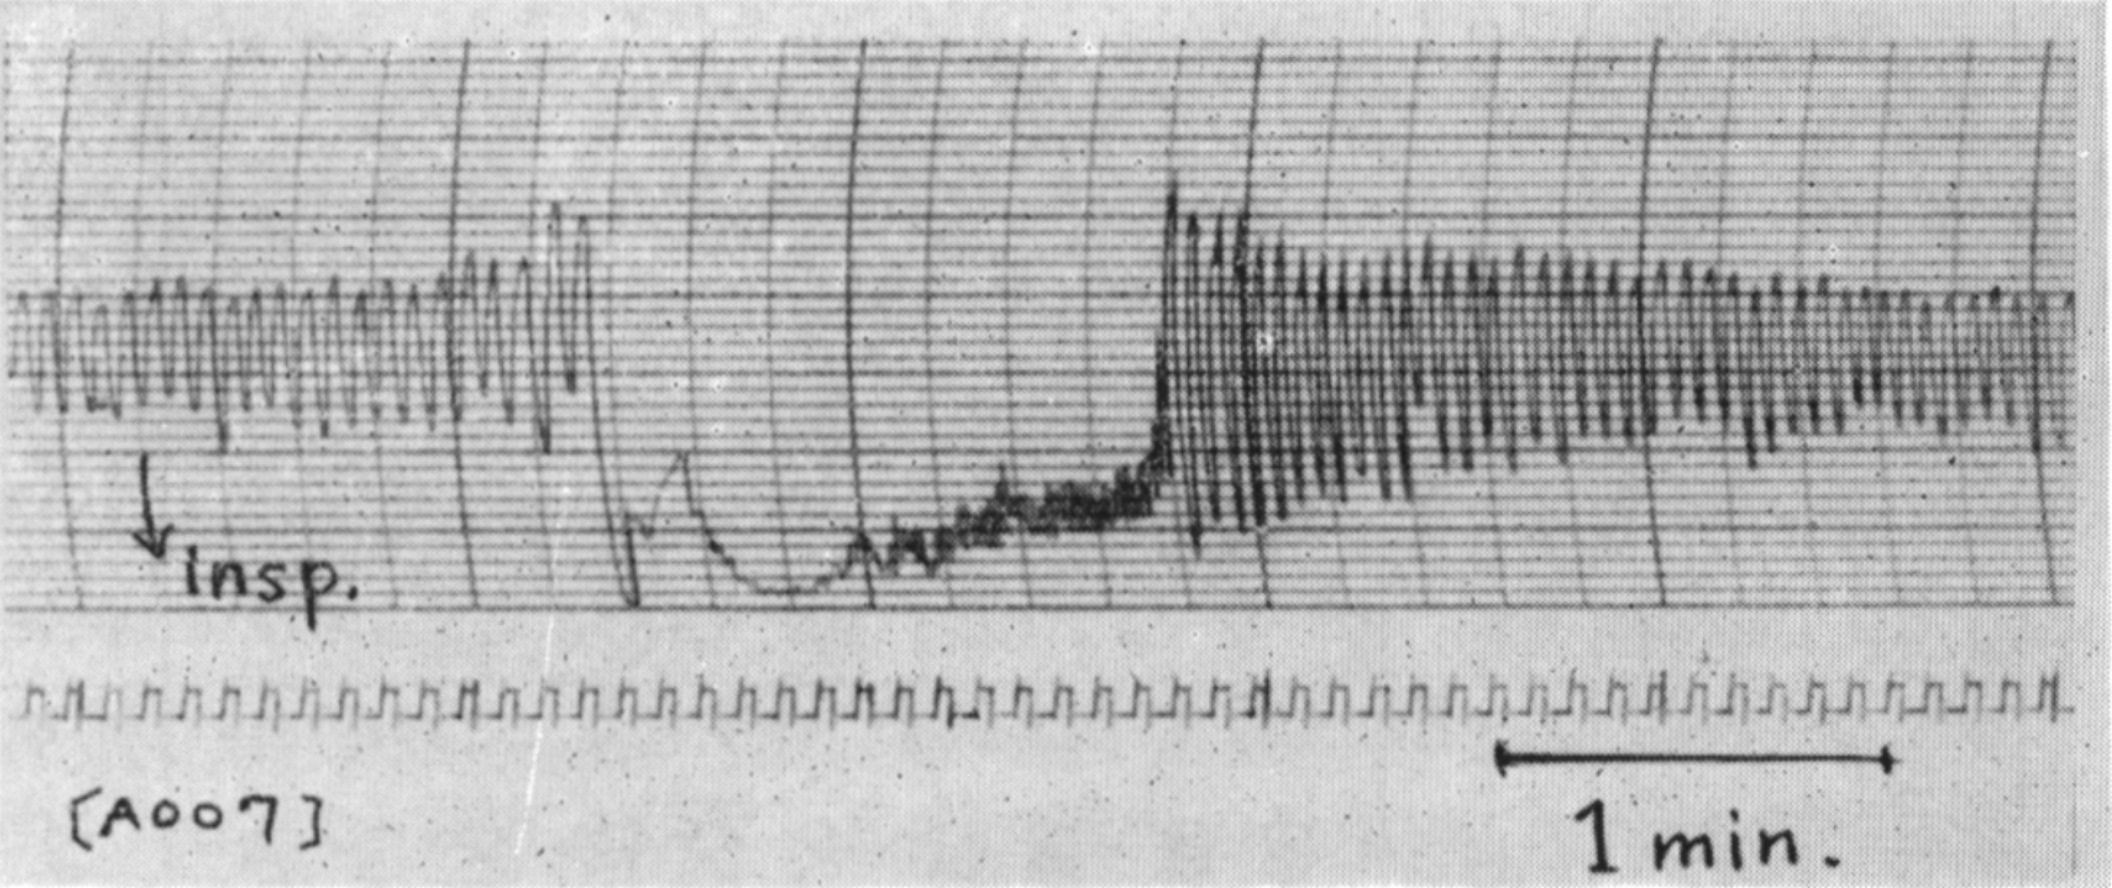
\includegraphics[width=0.66\textwidth]{images/respiration/respiration_regeneration}
    \caption{Regenerationsphase nach Luft anhalten \cite{beath_rebreathing}.}
    \label{fig_respiration_regeneration}
\end{figure}

\begin{figure}[ht]
    \centering
    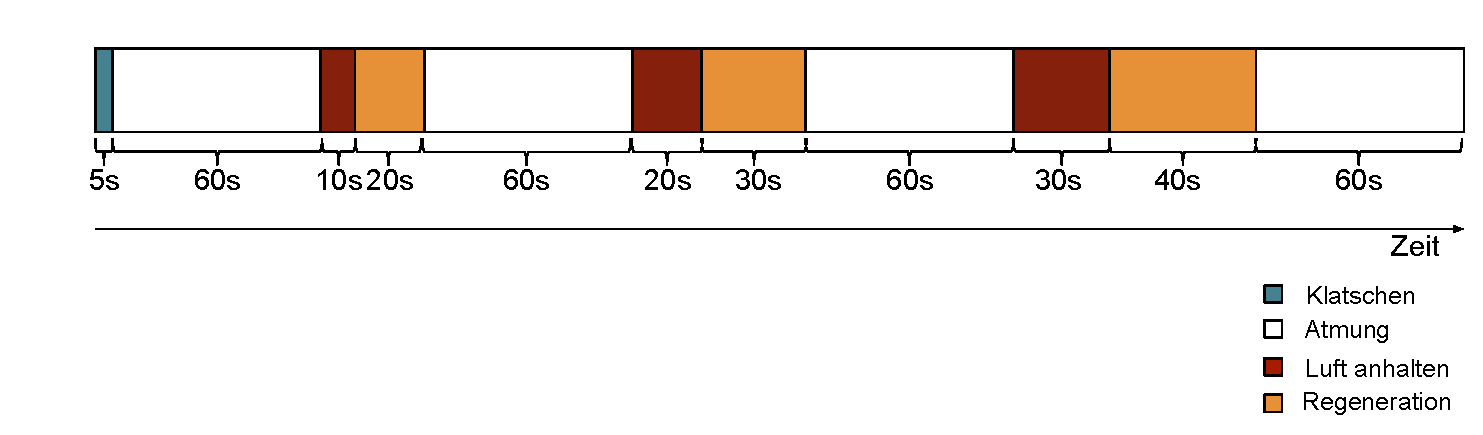
\includegraphics[width=1\textwidth]{images/study/study_flow2}
    \caption{Ablauf der Studie mit einer Position}
    \label{fig_study_flow}
\end{figure}

\section{Studienablauf}
Dieser Ablauf (siehe Abb. \ref{fig_study_flow}) wurde nun pro Studienteilnehmer jeweils bei den 3 Positionen durchgeführt, womit alle Schlaflagen abgedeckt wären.
Zu Beginn der Studie fand eine kurze Einweisung statt, indem der Proband erfuhr, was er zu tragen hat und wie er Anweisungen erhält, um dem Ablauf folgen zu können. 
Die Kamera wurde auf dem Stativ platziert und so ausgelegt, dass sie das Ohr des Probanden filmt. 
Das PSG-System wurde am Studienteilnehmer angebracht, sowie alle nötigen Sensoren, die im Kapitel \ref{ch:sa:psg} beschrieben wurden.
Nach der passenden Auswahl des Aufsatzes der eSense-Earpods war der Aufbau der Studie beendet.

Nun wird die Messung des PSG-Systems gestartet, sowie die Smartphone-App geöffnet. 
Nach Eingabe der Nutzerinformationen kann der erste Durchgang, welcher abhängig vom Ablauf der 3 Positionen war, begonnen werden.
Durch den Start der Messung am Smartphone beginnt die Messung. 
Da zusätzlich das Mikrofon am eSense-Earpod mit aufgezeichnet wird, wird nach dem Start der Messung ein $4\si{\s}$ Zeitfenster gewählt, indem der Teilnehmer in die Hände klatschen musste, um das Mikrofonsignal später synchronisieren zu können.
Nun beginnt die Aufzeichnung. Der Leiter der Studie hat bereits den Raum verlassen und alle Anweisungen werden durch die Earpods per Audiosignal ausgesprochen. 
Sofern die Messung beendet ist, tritt der Leiter der Studie wieder in den Raum und die Messung kann exportiert werden. 
Der Export beinhaltet jegliche Smartphone-Daten. Die PSG-Daten werden als eine komplette Messung am Ende der Studie exportiert.
Zudem wird die Kamera angehalten und eine neue Aufnahme kann gestartet werden.
Anschließend beginnt die nächste Position. Der Proband kann nun die neue Position einnehmen, anschließend wird per App die neue Messung gestartet.
Zum Abschluss aller 3 Positionen wird die Messung am PSG-System gestoppt und mittels eines vom PSG-System bereitgestellten Programms lässt sich die Messung als \glqq \textit{edf}-Datei\grqq exportieren.
Mehr zum Export der Daten und zur Synchronisation, siehe Kapitel \ref{ch:Implementierung:way_to_pipeline}
Pro Position dauert eine Messung ca. 7 Minuten, was bei 3 Personen eine Gesamtdauer von 21 Minuten bedeutet.
Einschließlich der Instruktionszeit, dem Export nach der Messung und den Positionswechseln der Probanden war die durchschnittliche Gesamtdauer einer Aufzeichnung ca 45-60 Minuten. 